
\section{The Milky Way and its stellar halo in the \textit{Gaia} era}

Next we cover the major advancements in the study of the Milky Way stellar halo that have been enabled by \textit{Gaia}. First will be covered the important observational campaigns that have produced data for these advancements, including \textit{Gaia} itself as well as ground-based spectroscopic and photometric projects which offer needed support. Then the major discoveries using these data will be covered, focusing specifically on the stellar halo. Finally, we will look ahead to problems that need to be solved, which will lay the groundwork for this thesis.

\subsection{Surveys of the \textit{Gaia} era}

As has been outlined in the previous sections, much theoretical work had been done since the advent of the $\Lambda$CDM paradigm and prior to \textit{Gaia} to understand the formation and evolution of galaxies. In reading many of these works, one is struck by how often \textit{Gaia} is invoked as the harbinger of the data that will be able to discriminate among competing hypotheses. In this section we will discuss the \textit{Gaia Space Telescope} as well as other observational efforts that have all provided crucial data both to explore the Milky Way and answer some of these theoretical questions of galaxy formation and evolution.

\subsubsection{The Gaia Space Telescope and scanning space astrometry}

% 6D phase space 
Fundamental to the study of stars in the Milky Way is knowledge of their 6D phase space coordinates, which are required to compute their positions and orbits. In our spherical frame of reference these six quantities take the following form: two on-sky positions, the distance to the star from us, its radial velocity along the line-of-sight, and two proper motions along the plane of the sky. Of these quantities, on-sky position is trivially obtainable with any photometric observations. The radial velocity of a star can be measured via the Doppler shift in its spectrum, which is more observationally demanding to obtain than photometry but still feasible and widely done. These three quantities have been determined for a large number of stars in the nearby Milky Way since, for example, the SEGUE project \parencite{segue} of the first Sloan Digital Sky Survey \parencite[SDSS;][]{sdss} in the early part of the 21st century began to mass produce stellar radial velocities.

% Distances and proper motions
There are a variety of ways to obtain stellar distances, and many are not particularly reliable. One can measure the properties of a star (such as surface temperature, gravity, colour, etc...) and estimate its absolute magnitude, thereby using the measurement of its apparent magnitude to derive a distance. While this is feasible for ensemble stellar populations such as open clusters or globular clusters, since all stars are expected to lie on a single isochrone, doing this for individual stars provides distance estimates rife with uncertainty. A more reliable distance measurement is a geometric one, leveraging the fact that the Earth orbits the Sun with a semimajor axis of 1~AU ($\sim 1.5 \times 10^{8}$~km) and using the resulting parallactic shift of nearby stars with respect to a distant background to compute distances. This requires precise positional measurements, which also happens to be the only way to compute the proper motion of a star in the plane of the sky.

% The measurement of parallaxes
Such measurements are challenging for standard ground- or space-based telescopes for a number of reasons. To obtain accurate parallaxes, multiple observations over the span of a year (or more) are needed and systematics associated with pointing errors need to be minimal. These requirements are such that for most ground-based telescopes and many space-based telescopes (the \textit{Hubble Space Telescope} is a noteworthy exception) it is either not worthwhile to perform these measurements (i.e. the field of view is small enough that very few stars would get measured parallaxes, yet multiple nights of observing would be needed) or the required precision is not obtainable (i.e. due to pointing systematics which are not an issue for the normal targets of the telescope). To work around these limitations, purpose-built space telescopes have been designed to measure parallaxes and proper motions for nearby stars.

% Hipparcos and scanning space astronometry
The HIPPARCOS space mission was the first of such facilities, operating in the early 1990s it was influential as the first observatory to mass-produce parallax and proper motion measurements \parencite{hipparcos}. Previous to HIPPARCOS the number of stars for which parallaxes were measured was $< 10^{4}$, and afterwards the number was raised to $> 10^{5}$. HIPPARCOS operates using the principles of scanning space astrometry \parencite[see][]{lindegren10}. To summarize: an astrometric space observatory can scan the whole sky by rotating about an axis which also precesses. What is unique, however, is that the canonical design employs two telescopes with fields of view separated along the scanning direction by a `basic angle', which must be a non-trivial fraction of $360\degr$. The crux of the two-telescope design is that by simultaneously making two sets of positional measurements systematic errors can be mitigated. By ensuring the basic angle cannot easily divide a great circle each positional measurement made in one field can be observed simultaneously alongside a range of other fields, and those fields can then be observed with other, mutually exclusive sets of fields, and so on. This allows for the construction of a `global' astrometric solution, whereby a rigid reference frame anchored by distant background sources is established in tandem to the astrometric solution for each star.

% Gaia
The \textit{Gaia} space telescope was launched in 2014, and continues to take observations to this day \parencite[see][ for design specifications and related references]{gaia}. It operates using the principles just described, but has some key improvements in design and operation when compared to its predecessor. The most pertinent of these are: two larger primary mirrors (HIPPARCOS used a single primary mirror with a beam combiner); a pair of photometers with modern CCD detectors which allow for broad-band photometry between $300-1000$~nm (HIPPARCOS had a photometer with a single band); and finally a spectrometer for radial velocity measurements (HIPPARCOS had no capacity to measure radial velocities). The observational capabilities of \textit{Gaia} are a major step beyond HIPPARCOS. It can measure parallaxes for $> 10^{9}$ stars ($10^{5}$ times more), with microarcsecond precision (versus milliarcsecond precision), and also obtain radial velocities for about $10^{7}$ bright stars (giving full 6D phase space information), and use its photometer to obtain the equivalent of very low-resolution spectra that can be used to derive temperature and abundance estimates. To give some approximate ranges of physical parameters corresponding to the \textit{Gaia} uncertainties: for stars of a typical brightness the distance at which parallax errors dominate is about $5-10$~kpc, and the nominal proper motion uncertainties correspond to velocities at these distances of $\sim~10$~km/s. Contrast this to HIPPARCOS, where the largest distances effectively measurable are only about 100~pc, with similar space velocity uncertainties (although obviously \textit{Gaia} is obtaining this similar velocity accuracy at much larger distances). This exquisite dataset has thus far exceeded expectations \parencite[e.g. see a commentary and review by][shortly after the second data release]{brown21}, and will act as the centerpiece of Milky Way science for the next generation: the \textit{Gaia} era.

% Limitations
But despite its success \textit{Gaia} is not the final word, and complementary observations to supplement some of the notable gaps and limitations of the \textit{Gaia} data are warranted. For example, \textit{Gaia} is only capable of limited abundance and stellar parameter estimates for very bright stars as the only truly resolvable spectral features it observes are the Ca II triplet and other nearby lines in the narrow radial velocity spectrometer window between $845-870$~nm (the photometric instrument is not capable of meaningfully resolving spectral features). Another limitation is that radial velocity measurements, although numerous, can only be obtained for bright, mostly nearby stars. Finally, although \textit{Gaia} does provide excellent photometry and astrometric parameters for $G < 21$\footnote{$G$ is the \textit{Gaia} integrated bandpass, spanning $\sim 300-1000$~nm.}, much of the Milky Way and nearby dwarf galaxies are fainter and can only be probed with more sensitive photometry even though that may lack astrometry. In the next section some of the supporting observations that bolster the \textit{Gaia} data will be introduced.

\subsubsection{Spectroscopic observations: chemistry and radial velocities}

% Introduction
The most important type of observations that complement \textit{Gaia} is ground-based spectroscopy. As noted above, \textit{Gaia} is somewhat limited in its ability to obtain stellar abundances or parameters using the radial velocity instrument. Therefore many projects have been undertaken to supply large amounts of spectroscopic data. These projects are not sparked solely by \textit{Gaia}, and spectroscopy has been important to the study of the Milky Way for many years, but it is now seen as an imperative to be able to fully exploit the data provided by \textit{Gaia}. Typically these surveys are ground-based, visible to near-infrared, medium- to high-resolution ($\mathrm{R} \sim 1,000-100,000$), and target between $10^{4}$ to $10^{6}$ stars. Obviously as astronomical resources improve due to the availability of new technology and new observatories, the resolution, wavelength coverage, and number of stellar targets all increase. A landmark early effort, and a template for later projects, is the Sloan Digital Sky Survey \parencite[][]{sdss}. A multi-faceted observational campaign which has existed now in five subsequent iterations over 24 years \parencite[see ][for the third and fourth generations]{sdss3,sdss4}, SDSS has provided spectroscopic and photometric observations of stars and galaxies over large parts of both the southern and northern sky.

% SEGUE and APOGEE
One of the first major stellar spectroscopic surveys was SEGUE \parencite{segue}, a component of SDSS-II, which obtained optical spectra for $\sim 240,000$~stars from which abundances and radial velocities could be derived. SEGUE allowed for the large-scale investigation of Milky Way disk structure, chemistry, and kinematics \parencite[e.g.][]{bovy12c,bovy12d,schonrich12,bovy13}, as well as the stellar halo \parencite[e.g.][]{smith09,xue11,kafle12,xue15}. Even though only radial velocity information is available from such a survey, modelling is still possible by marginalizing over tangential motions. The successor to SEGUE was the Apache Point Galactic Evolution Experiment \parencite[APOGEE;][]{apogee} of SDSS-III and SDSS-IV. APOGEE is different from SEGUE and many other spectroscopic programs in that it operated in the near-infrared ($H$-band). This allowed it to obtain better observations of the dust-obscured Galactic plane and the near-infrared is a wavelength domain rich in spectral features for useful elements including many $\alpha$, odd-Z, and iron-peak elements in addition to C and O. APOGEE, like SEGUE, has enabled the detailed study of the Milky Way disk and halo \parencite[see][for a few examples of noteworthy results]{bovy12a,hayden15,hayes18,mackereth19a}. SDSS, and APOGEE in particular, are emphasized here because these data are used in this thesis. Additional observational details will be presented in each chapter where relevant.

% Other spectroscopy 
Other important spectroscopic surveys have preceded both \textit{Gaia} and SEGUE/APOGEE, been performed contemporarily with them, or are to be expected in the future. Some examples of important past and present surveys include the Geneva-Copenhagen Survey \parencite{gcs}, \textit{Gaia}-ESO \parencite{gaiaeso}, LAMOST \parencite{lamost}, GALAH \parencite{galah}, RAVE \parencite{ravedr16}, H3 \parencite{h3}, and DESI \parencite{desi}. Surveys that have yet to be completed include 4MOST \parencite{4most}, WEAVE \parencite{weave}, and SDSS-V \parencite{sdss5}. These surveys each have different advantages and limitations, and observe different parts of the sky, and different stellar targets over different wavelength ranges. Combined, this gives the modern astronomer a wide range of different datasets to work with depending on the science objective. It is also worthwhile to point out though that while large-scale spectroscopic projects synergize better with \textit{Gaia}, spectroscopy on large or more sensitive telescopes (e.g. Gemini, \textit{Hubble}, Keck, VLT) can still be necessary to probe faint targets or to obtain the highest resolution, highest signal-to-noise spectra. An example where such an approach is necessary is the study of dwarf galaxies in the far outskirts of the Milky Way, the stellar constituents of which are often too faint to target as a part of large-scale projects. The downside of this approach is obviously that it can only be done for very few stars.

% Abundances and stellar parameters
The primary use for stellar spectra is to compute accurate stellar parameters (i.e. surface gravity, effective temperature) and, most importantly, elemental abundances. Most stellar spectra are sufficient to compute aggregate stellar parameters, but to obtain elemental abundances requires certain resolution and signal-to-noise thresholds be crossed. Moreover, as each element has a variety of absorption lines manifesting at different wavelengths, some spectral regions are better suited for different elements. For example, heavy metals tend to have their strongest absorption features in the blue end of the spectrum, meaning that GALAH (which has one blue spectral channel) is more sensitive to their abundances than APOGEE (which operates in the infrared). On the other hand APOGEE is less impacted by dust and can therefore probe a larger volume of the Milky Way. Another difference between these surveys is the areas of the sky they target, since spectroscopy is observationally expensive to obtain, most surveys do not cover the whole sky. For example, the H3 survey focuses on fields near the Galactic poles so as to study the stellar halo, while APOGEE contains a mix of fields oriented towards the disk, bulge, and Galactic poles. Similar trade-offs exist between spectroscopic programs in terms of resolution and sensitivity as well, and the overall emphasis is that a variety of parallel efforts are warranted to complement \textit{Gaia} and study the Milky Way from different perspectives.

% Deep learning and stellar properties
Another benefit of spectroscopy, especially on large scales, is that a spectrum contains extensive information about a star. This has lead to the emergence of a vibrant subfield of Milky Way astronomy focusing on the derivation of stellar parameters from spectra using increasingly novel methods. Such techniques are needed both to efficiently compute stellar properties for the large amounts of data, but also they can potentially exploit subtle spectral features and other correlations to accurately derive parameters that, at face value, do not seem as though they can be derived with a given spectrum. For example, a range of neural network architectures are now commonly used \parencite[e.g.][]{leung19a,leung19b,ting19}, in addition to more classic statistical techniques that directly fit the spectra \parencite[e.g.][]{ness15,queiroz18,cargile20}. These methods can be data-driven or model-driven, and often fold in other information such as \textit{Gaia} parallaxes, photometry, and theoretical isochrones and spectral templates. An example of how such techniques can be used to glean useful information beyond simple stellar parameters and abundances is the AstroNN framework of \textcite{leung19b}. Here, a deep neural network is trained on nearby APOGEE red giants with accurate \textit{Gaia} parallaxes, and then used to obtain distances to far away stars which are superior to the distances obtained by \textit{Gaia}. This is possible because the model is able to learn an analog of a star's absolute magnitude via its spectrum, since red giant stars manifest distinct changes in their spectra as they climb the red giant branch. Another good example is how neural networks may be trained also to derive stellar ages (actually the mass, which is directly linked with the age) for giants by using C and N abundances as a proxy \parencite{leung23}. The abundances of these elements are modified in a mass-dependent manner for red giants as the star undergoes convective dredge-up \parencite{martig16}. A final recent example is the emergence of so-called `foundation models', which aim to comprehensively learn about and predict a variety of stellar properties (although such models are not limited to stars) using transformer neural network architectures, and the embedding and attention mechanisms that characterize them \parencite[e.g.][]{leung24}. Such models may be capable of taking in a huge range of astronomical data and predicting an equally wide range of stellar parameters and properties. These are just a few examples of how modern statistical techniques are being applied to astronomical observations, and stellar spectra in particular, to substantially amplify the power of the data.

\subsubsection{Photometric observations and other complements to \textit{Gaia}}

% Introduction
A final set of observations to cover in the context of \textit{Gaia} and the Milky Way is deep photometry. While \textit{Gaia} does obtain photometry itself, it is limited in its ability to probe fainter stars and structures (limiting magnitude of $G \sim 21$). There is therefore scope to supplement what can be learned with \textit{Gaia} using more sensitive photometry. Examples of such programs past and present include earlier SDSS iterations \parencite[which lead to the already-noted `field of streams';][]{belokurov06}, Pan-STARRS \parencite{panstarrs}, DES and its offshoots \parencite{des}, CFIS \parencite{cfis}, and the older but crucial infrared survey 2MASS \parencite{2mass}. Deep all-sky photometry, especially over multiple bands from the blue to near-infrared, allows for meaningful study of the Milky Way even though one cannot typically derive the individual stellar parameters which require spectra. Colours are useful metrics to study aggregate stellar populations, since they are sensitive to age and overall metallicity. Populations arising from a single bout of star formation, such as globular clusters or even small dwarf galaxies, will lie upon an isochrone as long as the stars are at approximately the same distance. This can make photometry useful for detecting stellar streams \parencite[e.g.][]{odenkirchen03,grillmair06,belokurov06,bernard14}, as well as dwarf galaxies such as the Sgr dwarf spheroidal discussed in the previous section \parencite{ibata94}.

% Other stuff
A few other styles of observatory or observational program are worth quickly noting for their use in the study of the Milky Way. First are stellar asteroseismic studies, which link pulsation-induded changes in stellar luminosity to their interior properties \parencite[see][for a review]{kurtz22}, and allow for the computation of stellar masses (and therefore ages). Asterosiesmology requires short-cadence, sensitive photometry, and is therefore naturally done by space-based telescopes hunting for planets via the transit method, such as \textit{Kepler} \parencite{kepler} or TESS \parencite{tess}. Ages are a crucial property for a star, and future work to derive ages using spectra (see above) and known asteroseismic ages as training information will certainly be fruitful \parencite[e.g. see][]{montalban21}. The second style of observation is narrow-band imaging, which typically use a very narrow photometric filter centered on a prominent spectral feature to perform photometry over a large part of the sky. The idea is that metal-poor stars, for example, will appear in stark contrast when the photometry using this special filter is contrasted (i.e. a colour) with other wide-band photometry. Since such observations are easier to obtain over the whole sky compared with spectroscopy, this is an easy way to farm large numbers of metal-poor stars. Examples of such projects are the Pristine survey on the CFHT \parencite{pristine} and the Southern Sky Survey on the SkyMapper telescope \parencite{skymapperdr1}. The third style of observation are purpose-built low-surface brightness facilities, which are able to image the faintest luminous components in the nearby Universe. A good example of such an observatory is the Dragonfly Telephoto array \parencite{dragonfly}, which uniquely uses commercial cameras with special optics and detectors that reduce scattered light. Dragonfly has discovered some of the most enigmatic \parencite[i.e. both lacking, and being completely dominated by dark matter;][]{vandokkum16,vandokkum18}, lowest surface brightness galaxies yet known \parencite{vandokkum15}, opening up a wide range of new opportunities and challenges for galaxy formation theory.

% Upcoming facilities
Finally, upcoming facilities, which ostensibly have other goals beyond Milky Way science, will also play a large role in the study of the faint outskirts of the Milky Way. Most notable is the Rubin observatory \parencite{lsst}, which will perform multi-band photometry of the entire southern sky on a weekly basis. The limiting magnitude of the co-added images is expected to be $r \sim 28$, much fainter than other surveys that have mapped a comparable amount of the sky. \textit{Euclid} and \textit{Roman} are two space telescopes which will begin operations soon (\textit{Euclid} has launched and is obtaining data, \textit{Roman} is expected to launch in 2026), performing photometry and spectroscopy from the middle of the visible spectrum to the near-infrared. While their primary science goals are extragalactic in nature, they (will) have wide fields of view and excellent space-enabled resolution and sensitivity which will allow for the study of faint stellar populations in clusters and other areas of interest around the Milky Way. Another area of research that will be opened up by these three facilities is the study of stellar halos around other galaxies in the nearby Universe, which are challenging to probe owing to their faintness and low surface brightness. This will hopefully open up new avenues to study (extra)galactic archaeology in the same way that has been done for M31 with surveys such as PandAS \parencite{mcconnachie09}. The \textit{James Webb Space Telescope} also has an important role to play in the study of the formation and evolution of galaxies, in that it can probe the high-redshift epochs of the assembly and growth of the first galaxies that resemble the Milky Way.

\subsection{Major discoveries in the stellar halo}

% Brief introduction to the subsection
We have seen that \textit{Gaia} and the complementary observations that bolster it have created a rich, multidimensional dataset. Now the discoveries made in this new era will be summarized, focusing on those which are important for the work that will be presented in this thesis. For more detail, and a broader look at the impact on the stellar halo from \textit{Gaia}, two good recent reviews have been written by \textcite{helmi20} and \textcite{deason24}. As an accompaniment to the discussions in this section, we show a sample of metal-poor stars from APOGEE DR17 in Figure~\ref{ch1:fig:APOGEEDR17_spatial_abundances} and Figure~\ref{ch1:fig:APOGEEDR17_kinematics}. See the caption of the first of those for the specific selection criteria. Figure~\ref{ch1:fig:APOGEEDR17_spatial_abundances} shows the spatial distribution of the stars in Galactocentric coordinates as well as [Fe/H], [Mg/Fe], and [Al/Fe] abundances. Figure~\ref{ch1:fig:APOGEEDR17_kinematics} shows the kinematics of the stars, including velocities, angular momentum, eccentricity, energy, and radial action.

\subsubsection{\textit{Gaia}-Enceladus, remnant of the last major merger?}

% Discovery of GS/E by Belokurov
The first \textit{Gaia} data release only contained positions for most stars \parencite{gaiadr1}, with just a small subset of nearby stars having parallaxes and proper motions (mostly those overlapping with HIPPARCOS), but some creatively combined the available \textit{Gaia} data with archival SDSS data to compute rough (largely photometric) distances and proper motions to a larger sample \parencite{deason17,deboer18}. \textcite{belokurov18} presented an analysis of the anisotropy of the stellar halo using these data, finding that the anisotropy increased markedly as [Fe/H] increased. The low-metallicity halo ($\mathrm{[Fe/H]} < -2$) had an anisotropy of $\beta \sim 0.3$, which is not unexpected value, but the metal-rich halo (up to $\mathrm{[Fe/H]}=-1$) had anisotropy values as high as 0.9. They found this high-metallicity population to comprise roughly half the nearby stellar halo, and exhibit modest net rotation. Drawing on zoom simulations, they concluded that the most likely origin of this metal-rich high-anisotropy stellar halo population was a single, massive ($\sim 10^{11}$~\Msun) accretion event long ago. Since this population of stars, when examined in velocity space, is elongated in the radial velocity direction and contracted in the tangential velocity direction they named the purported remnant `The Sausage' (see Figure~\ref{ch1:fig:APOGEEDR17_kinematics}).

\begin{figure}
    \centering
    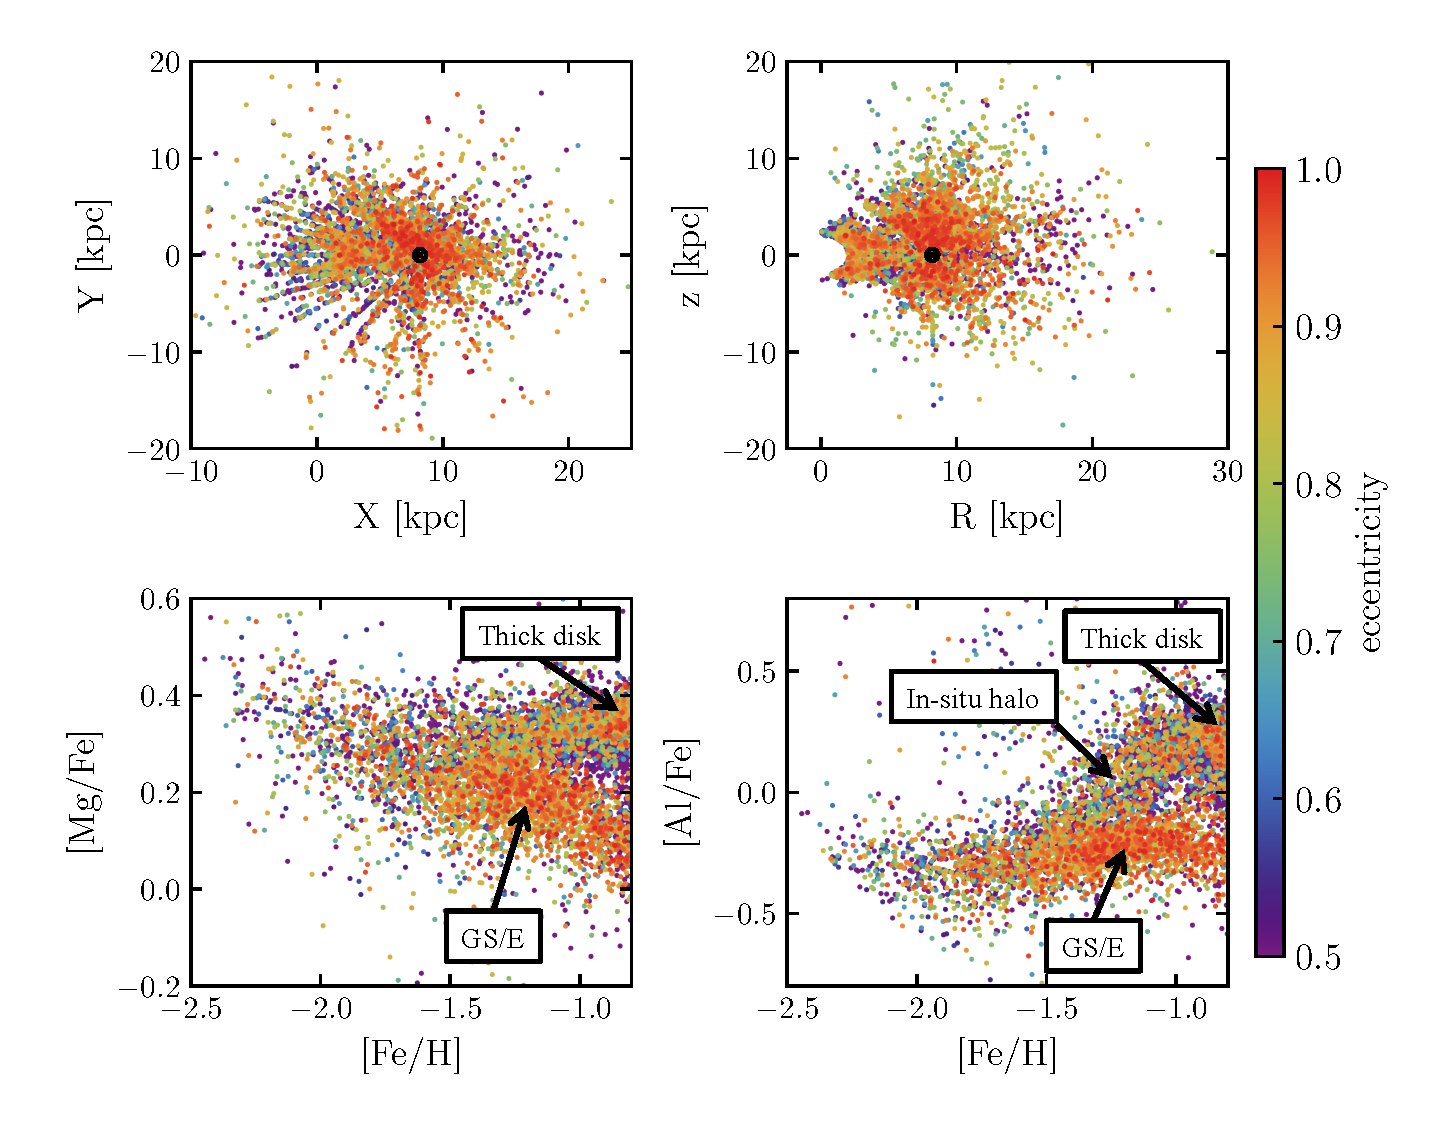
\includegraphics[width=\textwidth]{figure/ch1/apogee_dr17_spatial_abundances.pdf}
    \caption{A sample of APOGEE DR17 stars selected from the main survey according to the following criteria: [Fe/H]$< -0.8$, $1 < \log g < 3$, $r_\mathrm{GC} > 2$~kpc, and [Mg/Fe] and [Al/Fe] must be measured. Major stellar populations are annotated to guide the reader. \textit{Top left:} Galactocentric X and Y coordinates, the position of the Sun is marked. \textit{Top right:} Galactocentric cylindrical radius and height above the disk, again the position of the Sun is marked. \textit{Bottom left:} [Mg/Fe] abundance as a function of [Fe/H] abundance. The metal-rich (for halo stars) GS/E remnant is marked along with the metal-poor part of the high-$\alpha$ disk. \textit{Bottom right:} [Al/Fe] abundance as a function of [Fe/H] abundance. GS/E and the thick disk are again marked, and the \textit{in-situ} stellar halo at intermediate [Al/Fe] abundance is also shown.}
    \label{ch1:fig:APOGEEDR17_spatial_abundances}
\end{figure}

\begin{figure}
	\centering
	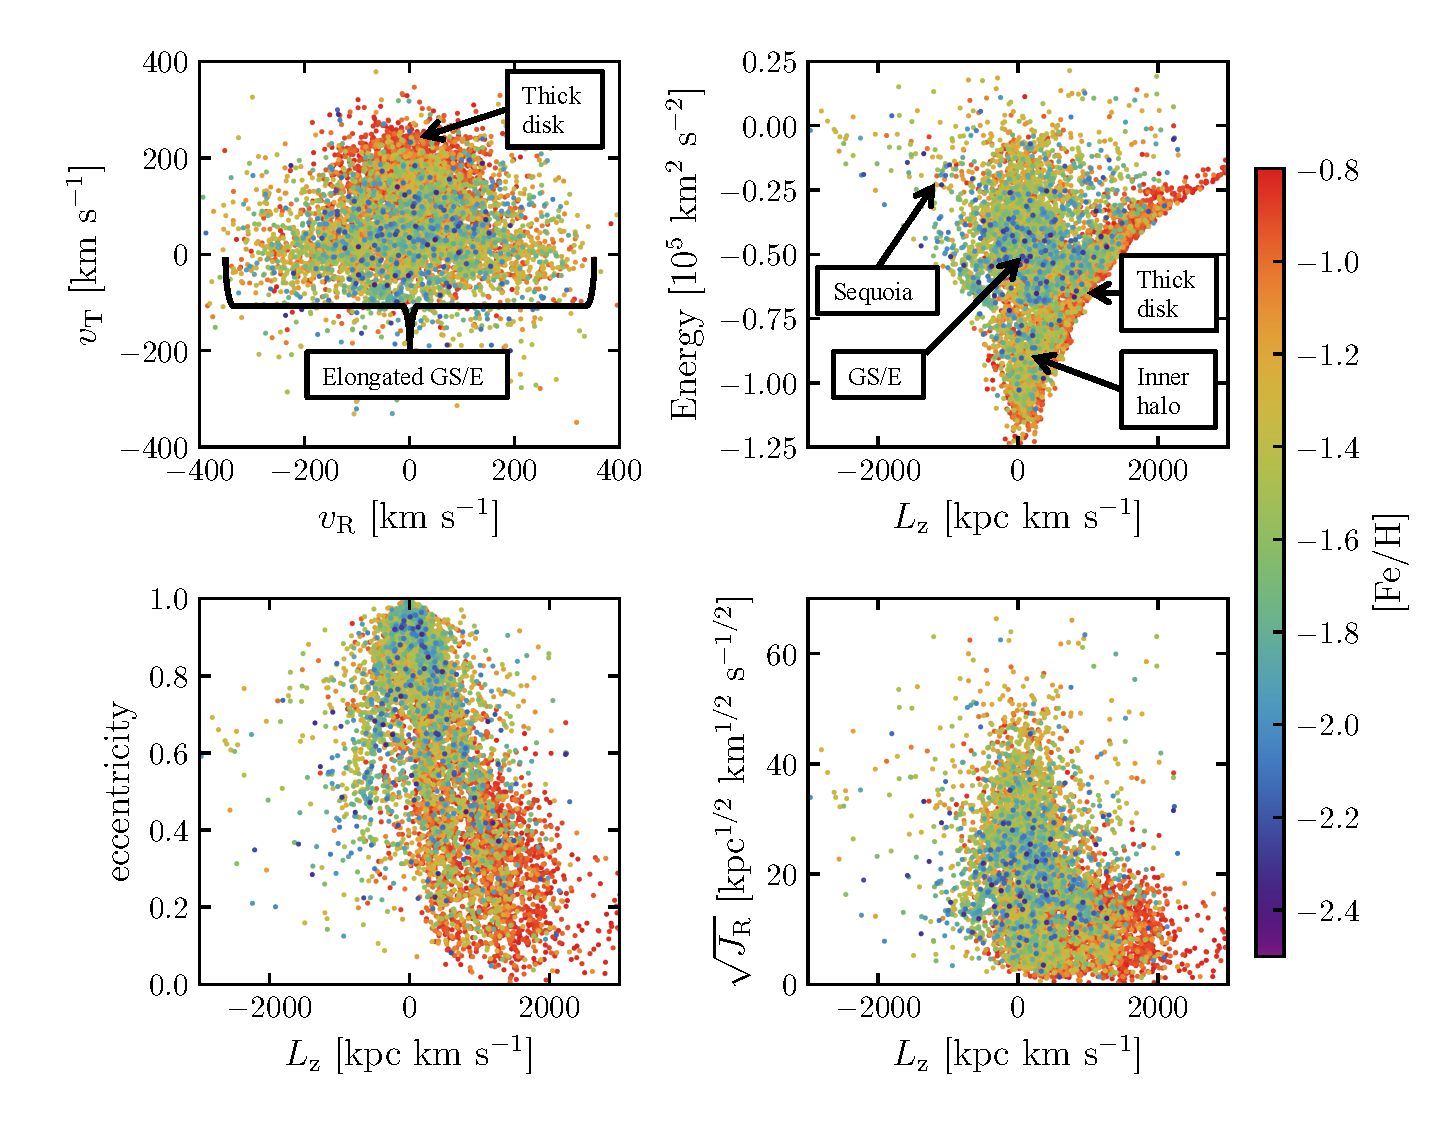
\includegraphics[width=\textwidth]{figure/ch1/apogee_dr17_kinematics.pdf}
	\caption{The kinematics of the same APOGEE DR17 samples as shown in Figure~\ref{ch1:fig:APOGEEDR17_spatial_abundances} coloured by [Fe/H]. Major stellar populations are again annotated. \textit{Top left:} Galactocentric cylindrical tangential velocity as a function of radial velocity. Offset at positive tangential velocity, the metal-poor part of the thick disk is marked. The velocity ellipsoid of the GS/E remnant is elongated in the radial direction, which is how it gets the name `sausage'. \textit{Top right:} Energy as a function of angular momentum. GS/E is visible as a cloud of low-angular momentum debris at higher metallicity. The locus of the high-energy, retrograde Sequoia remnant is shown, but it is not numerically significant in the APOGEE data. The inner halo, likely containing much of the \textit{in-situ} halo, is shown at low energy. \textit{Bottom left:} eccentricity as a function of angular momentum. \textit{Bottom right:} square root of the radial action as a function of angular momentum. In these final two panels GS/E is clearly visible as the cloud of higher metallicity debris with high eccentricity and radial action respectively.}
	\label{ch1:fig:APOGEEDR17_kinematics}
\end{figure}

% Additional measurements: Myeong, Haywood, and Helmi
The most important release of \textit{Gaia} data was the second data release in April 2018 \parencite{gaiadr2}, which provided parallaxes and proper motions for most of the planned survey volume to a community eager to further study the Sausage. \textcite{haywood18} studied the twin colour-magnitude diagram tracks of high proper motion stars presented by \textcite{gaiadr2_hrdiagram}, finding that the red sequence is consistent with the thick disk and the \textit{in-situ} halo, while the blue sequence is consistent with a single accreted population with particularly eccentric kinematics: the Sausage. \textcite{myeong18} study globular clusters with integrals of motion consistent with the Sausage population, finding a distinct group with such properties that also lies along a single track in the age-metallicity plane, as globular clusters formed in a single galaxy are wont to do. \textcite{helmi18} also expand the picture by studying the ages, energy, angular momentum, and [$\alpha$/Fe] of the metal-rich radial halo population. They definitively claim that this population arose from a single accretion event, which they name `'\textit{Gaia}-Enceladus', and further claim that it must have played a role in the formation of the thick disk. Hereafter this remnant will be referred to as \textit{Gaia}-Sausage/Enceladus (GS/E), as is now standard\footnote{This name has caused much consternation in the community, with many astronomers exasperated at the notion that the Sausage will be the name of this remnant, for understandable reasons. JL happens to quite like the name, and having given many public talks that include it as a topic, can vouch for the fact that the name is always received as funny and memorable.}. \textcite{deason24} provides a detailed accounting of the discovery process for GS/E for those interested.

% History of possible GS/E discoveries
Before moving on to discuss the flood of subsequent work on GS/E, it is also worth recognizing that many other previous works had hinted at the presence of GS/E. The stellar halo radial density profile was understood to be broken \parencite{deason11,sesar11}, with many observed overdensities coinciding with the break radius and potentially indicating apocenter pile-ups of an accreted dwarf \parencite{li16}. The halo was observed to have dual chemistry \parencite{carollo07,nissen10}, and the supposedly accreted component was understood to be chemically distinct from extant low-mass dwarf satellites \parencite{venn04}. Many of these works discuss the possibility of a large single merger event being responsible for their findings, and \textcite{deason13} directly investigate this hypothesis. Even just prior to the second data release of \textit{Gaia} several studies had demonstrated bimodalities in the stellar halo that could be interpreted as evidence for GS/E \parencite{bonaca17,deason17,hayes18}. The discovery of GS/E nonetheless nicely frames the pre-\textit{Gaia} discussions of the duality of the stellar halo as discussed in the previous sections.

% Ongoing efforts to characterize, velocity dispersion profile
After the initial studies cemented the reality that GS/E composes a large fraction of the nearby stellar halo, the task changed from discovery to interpretation and characterization. Further studies approached this from a variety of perspectives, including: kinematics and spatial distributions, abundances and the colour-magnitude trends, globular clusters, and theoretical considerations. The anisotropy trends observed by \textcite{belokurov18} have been spatially extended by \textcite{lancaster19}, who use Gaussian mixtures to trace the high and low anisotropy halo components to large distances with blue horizontal branch stars. Other studies looking at the anisotropy profile using similar approaches produced similar findings \parencite{necib19,bird19}. \textcite{deason18} measure the apocenters of the metal-rich, anisotropic halo stars, finding them to be typically 20~kpc, broadly in line with the halo break radius found by earlier studies \parencite[e.g.][]{deason11,sesar11,xue15}. This is consistent with the single major merger hypothesis in so far as most of the remmant stars in the inner halo will share a common apocenter which reflects the final apocenter of the progenitor system before full disruption \parencite[indeed, this was the driver for the hypothesis of][]{deason13}, leading to a prominent break in the density at that radius. 

% GS/E geometry and density profile
Geometrically, the inner halo where GS/E dominates has been observed to be ellipsoidal, and tilted with respect to the Galactic Center-Sun line, as well as the Galactic plane \parencite{iorio19}. The poles of the distribution align nicely with two previously discovered stellar halo structures: the Hercules-Aquila cloud and the Virgo Overdensity, which backed up the earlier hypothesis of \textcite{simion19} that these structures were manifestations of GS/E apocenter pileup, akin to the stellar halo break but for an ellipsoidal stellar distribution. Both \textcite{koppelman18} and \textcite{feuillet20} build on the earlier results of \textcite{helmi18} and \textcite{myeong18} and demonstrate that the characteristic kinematics of GS/E are reflected well by characteristic distributions in integrals of motion space, namely energy, eccentricity, angular momentum, and the radial action. Finally, \textcite{mackereth20} directly fit density profiles to mono-abundance populations of halo stars including a kinematically-selected GS/E population. They find that GS/E may only consist of roughly a third of the mass of the stellar halo in aggregate, somewhat less than other studies focused on the solar neighbourhood have found.

% Chemistry
Chemically, GS/E seems consistent with the remnants of a massive dwarf galaxy \parencite{fernandezalvar18,vincenzo19,monty20,hasselquist21}. See Figure~\ref{ch1:fig:APOGEEDR17_spatial_abundances} for some example abundances. Its star formation history seems to have been rapid and truncated, in line with expectations for a short-lived dwarf that likely spent most of its life in close proximity to the Milky Way. But complicating the picture is evidence that GS/E is enhanced in $r$-process elements \parencite{aguado21,matsuno21}. Such observations, along with other chemical analyses \parencite{sanders21}, seem to suggest that GS/E was the subject of non-standard enrichment vectors such as neutron star mergers or sub-Chandrasekhar Type Ia SNe, which could cloud or bias the inferences from earlier work that used more standard chemical evolution models \parencite[on which basis][ argues against a rapid and truncated chemical enrichment]{sanders21}.

% Globular clusters
Supporting these observations are those of globular cluster systems following the earlier work of \textcite{myeong18}. Such works typically examine globular clusters in terms of integrals of motion, age, and abundances, quantities each that are readily obtainable over the whole volume of the Milky Way. Most studies agree that the accreted globular cluster population could be described as being descended from a single major merger \parencite{massari19}, yet stress the potential importance of other mergers in the assembly history of the Milky Way as well \parencite{myeong19,kruijssen19b,forbes20}. Owing to their ability to trace the entirety of the stellar halo, and in contrast to early \textit{Gaia} results which focus on studying the halo in the solar neighbourhood, the fact that globular cluster data hints at a complex picture for the accretion history of the Milky Way should be taken as forewarning that expanding stellar catalogues will tell a similar story.

% Simulations
The final facet of study that helped to elucidate the nature of GS/E, and perhaps the most informative, is theoretical work focusing on N-body simulations. \textcite{fattahi19} solidify the standard narrative of a single major merger event by identifying high-anisotropy stellar halo populations in Milky Way analogs of the AURIGA simulation suite \parencite{grand17}, finding that they almost always are sourced from a head-on, early collision with a massive dwarf galaxy. These authors find that only about a third of Milky Way analogs have experienced such a merger. Interesting works that bridge the disciplines of globular clusters and N-body simulations is that of \textcite{kruijssen19b} and \textcite{kruijssen20}, who examine the simulated populations of globular clusters in the E-MOSAICS simulation \parencite{kruijssen19a}, and find evidence both for GS/E as well as many other remnants. Another influential study was that of \textcite{mackereth19a}, who search through Milky Way analogs in the EAGLE simulations using both dynamical and chemical information about GS/E to find more direct matches for the remnant, and therefore information about the progenitor. They are able to predict both an epoch for the event ($z < 1.5$) and a more accurate stellar mass ($\sim 10^{8.5-9}$~\Msun) than many of these other early works. \textcite{naidu21} employ tailored observations to try and match simulated GS/E merger events with observations from the H3 survey. They are able to predict both the stellar mass of the event ($4-7 \times 10^{8}$~\Msun) and the geometry of the encounter, linking their results with the findings of \textcite{simion19} and \textcite{iorio19}. Much of this work ties nicely into the pre-\textit{Gaia} work of \textcite{amorisco17} and \textcite{jean-baptiste17} who study the properties of tailored merger simulations around the Milky Way and develop solid formalisms that help to understand the observed clumping of accretion remnants like GS/E in integrals of motion space, as well as the radialization of their orbits on infall which also likely helped to shape the GS/E event. But it is also worthwhile keeping in mind the advice of \textcite{jean-baptiste17}, that the GS/E debris is likely very complicated in nature, and reconstructing the simple narrative of a single major merger may be challenging.

% Mass of GS/E
Observationally, the kinematics and chemistry of GS/E are now well understood on the basis of the large overdensity seen in the nearby stellar halo. The question now turns to learning more about the progenitor system of the encounter: how massive was it and at what epoch did it merge? With regards to the mass, a very wide range of values have been reported since the discovery of GS/E. \textcite{belokurov18} suggest the virial mass of the progenitor halo was $> 10^{10}$~\Msun, which is similar to estimates by \textcite{das20}. Using chemical evolution and star formation models, \textcite{helmi18}, \textcite{vincenzo19}, and \textcite{feuillet20} predict stellar masses in the range of $6\times10^{8} - 7\times10^{9}$~\Msun. Globular cluster-focused studies tend to estimate the mass to be slightly lower, between $2.7\times10^{8}-8\times10^{8}$ \parencite{kruijssen20,forbes20}. \textcite{mackereth20} estimate the mass to be $\sim 3\times10^{8}$~\Msun, and \textcite{naidu20} and \textcite{naidu21} estimate the mass to be in the range $4-7\times10^{8}$~\Msun. These later two constraints are on the low-end compared with other estimates, yet must be taken seriously since they are estimates based on direct star counts as opposed to an indirect modelling. The simulation-based work of \textcite{fattahi19} and \textcite{mackereth19a} suggests that in the cosmological context, GS/E can be expected to have a stellar mass in the range of $10^{8.5}-10^{10}$~\Msun, which is in line with most observationally-driven estimates.

% Accretion epoch of GS/E
Now with regards to the merger epoch of the remnant, a similar degree of uncertainty is also found in estimates. The strongest constraints on this timeline come from chemistry, since the star formation history of the progenitor is expected to cease as it begins infalling. \textcite{vincenzo19} and \textcite{sanders21} find that star formation histories extending for 3-4~Gyr match the data, placing the accretion time at about 10-11 Gyr in the past. This matches estimates of \textcite{helmi18} who consider a range of feasible isochrones for the associated stellar populations. Simulations back up these claims, and \textcite{fattahi19} and \textcite{mackereth19a} both estimate accretion redshifts of $z \sim 1.5-2.5$. A fantastic observational anchor is the work of \textcite{montalban21}, who use asterosiesmology to directly estimate the ages of member GS/E stars, finding they range from $8-12$~Gyr old, and therefore placing an estimate of the merger epoch at about 8~Gyr ago. \textcite{gallart19} make similar claims that the merger occurred about 8-10~Gyr ago based on isochronal ages for possible GS/E and thick disk stars. Synthesizing this information with the mass estimates above, and accepting canonical redshift-dependent stellar mass to halo mass relations where appropriate \parencite[e.g.][]{read17}, these GS/E mass and accretion timing estimates imply a mass ratio (GS/E to Milky Way mass at accretion) for the merger somewhere in the range of 1:2 to as low as 1:20.

% Why is knowledge of mass and age important
The reason that such questions are important is that GS/E could have constituted a major or a minor merger depending on these specifics. As thoroughly outlined in previous sections, major mergers form some of the core building blocks of galaxies such as ours, and therefore it behooves us to learn as much as we can about GS/E if it is indeed the most recent (or indeed largest ever) major merger. Some have hypothesized that GS/E was responsible for the creation of the thin-thick disk dichotomy, because the merger would have heated an existing stellar proto-disk and provided a new reservoir of gas for a subsequent generation of star formation \parencite{helmi18,gallart19}. These claims are made on the basis that the supposed epoch for the GS/E merger aligns with the typical ages of thick disk stars, and also such a mechanism has been theoretically studied as a thick disk formation scenario \parencite[e.g.][]{quinn93,purcell10}. Not only would this event then have created thick disk, but the most perturbed part of the early Milky Way could go on to form the \textit{in-situ} component of the stellar halo \parencite{haywood18,dimatteo19,belokurov20}, which is indeed observed to share many properties with the thick disk. These ideas naturally generate other hypotheses. Perhaps GS/E could have reset the metallicity of the disk, generating the high/low $\alpha$ dichotomy we see today? Could GS/E be responsible for the creation of the Milky Way bar \parencite{fragkoudi20}? How should we interpret the surviving Milky Way satellite population in the context of $\Lambda$CDM and a Milky Way with a GS/E-centric accretion history \parencite{bose20}? Such questions rely naturally on detailed knowledge of the properties of the progenitor to properly gauge its impact. GS/E could both be responsible for everything or nothing that occurred in the Milky Way in its early stages depending on its size and the timing of the merger.

\subsubsection{The rest of the stellar halo}

% Introduction, Helmi streams and Sequoia
While GS/E is the most prominent revelation thus far in the stellar halo, \textit{Gaia} has lead to quite a few other breakthroughs. The most interesting of these has been the discovery and characterization of a myriad of other unique stellar halo populations, many likely being merger remnants and some undoubtedly being part of the \textit{in-situ} halo. The Helmi Streams \parencite{helmi99} have been subject to deeper study with the new data and their nature as a likely low-mass merger remnant has been asserted \parencite{koppelman19a}. After GS/E, the most strikingly obvious apparent merger remnant is the so-called Sequoia feature\footnote{This name being adapted from the colloquial name for one of its likely constituent globular clusters: FSR 1758}, first discovered in globular cluster data by \textcite{myeong19}. The Sequoia is a retrograde high-energy group of stars originally suspected to be associated with GS/E \parencite{helmi18}, but shown to be unique in terms of the globular clusters and stars that trace it. The genesis of the discovery lies in  study of two peculiar retrograde star clusters: $\omega$~Cen, which has long been thought to be the nucleus of an accreted dwarf galaxy which has contributed retrograde debris \parencite{bekki03,majewski12}, and FSR 1758 about which similar questions have been raised \parencite{froebrich07,barba19}. The Sequoia has been subsequently (and unknowingly previously) studied by other authors using stellar and globular cluster data and confirmed to be a unique and separate halo population \parencite{koppelman19b,matsuno19,kruijssen20,monty20,naidu20}. The region of energy and angular momentum space occupied by Sequoia is noted in Figure~\ref{ch1:fig:APOGEEDR17_kinematics}, although there are insufficient stars to properly visualize it with APOGEE.

% The Kraken and Koala
Two supposed remnants have also been identified based on their associated globular clusters. \textcite{kruijssen19b} claim that the Milky has experienced 2--3 major mergers based on a comparison of the age-metallicity relation of Milky Way globular clusters with simulated analogs in the E-MOSAICS project \parencite{kruijssen19a}. By their measure, two of these events are accounted for by the ongoing merger of Sgr as well as GS/E, and an as-yet unidentified merger accounts for the third event, which exists today as a low-energy (inner halo) remnant they name the `Kraken' \parencite{kruijssen20}. But \textcite{massari19} argue that the clusters supposedly belonging to the Kraken are not dynamically coherent in a way that suggests a common origin, but multiple accretion events. \textcite{forbes20} also identify these low-energy clusters as arising from a single progenitor system, which they name the `Koala'. In Figure~\ref{ch1:fig:APOGEEDR17_kinematics} these remnants would occupy the low-energy part of the distribution of halo stars. The issue with studying the Kraken/Koala feature is that at low energy accreted clusters can be confused with \textit{in-situ} clusters, especially in regard to their kinematics, and so additional scrutiny is required to validate this discovery, preferably using stellar tracers.

% Stellar data
Indeed stellar data has been used to claim the discovery of multiple additional stellar populations, potentially indicating merger remnants. \textcite{koppelman19b} identify a low-energy, slightly retrograde group of stars with distinct kinematics and metallicities they name `Thamnos'. This group is likely very low mass, and could potentially be affiliated with the Sequoia structure, even though the energies of the two group are different. \textcite{naidu20} perform a very ambitious decomposition of the stellar halo using H3 data combined with \textit{Gaia} data. They identify Sgr and GS/E as the dominant stellar constituents of the halo, and confirm the identity of Thamnos and the Helmi Streams. But added to the picture are: a high energy, strongly co-rotating population they name `Aleph'; an intermediate energy, weakly co-rotating structure with similar kinematics to GS/E named `Wukong'; and they claim that the Sequoia hides two additional structures with similar kinematics but differing metallicity they call `I'itoi' and `Arjuna'. Combining these new and existing stellar halo populations and accounting for the hottest part of the Milky Way thick disk they claim that 95~per~cent of halo stars are contained within one of these structures, and that there is essentially no underlying smooth halo component. \textcite{horta21a} identify a distinct group of low-energy, low [Al/Fe] (indicating formation in a low-mass system) halo stars with minimal rotation and which is separate from GS/E. They call this `Heracles', and posit that it could be a fundamental building block of the Milky Way, similar in many respects to the Galactic bulge. The difference between this low-energy structure and the Koala/Kraken structures are debated, it could be that they are the same, or that Heracles is a genuine fundamental building block of the proto-galaxy while the Koala/Kraken reflect an early merger.

% The splash 
Up to this point the discussion of \textit{Gaia} discoveries has mostly revolved around claimed accretion remnants. But it is worth revisiting the \textit{in-situ} halo as well, and build on the discussion of its possible connection with GS/E. An excellent study of a new type of stellar population lying at the interface between the thick disk and the stellar halo was presented by \textcite{belokurov20}. They identify a population of metal-rich, high [$\alpha$/Fe], eccentric, weakly-rotating, flattened, old ($10-12$~Gyr) halo stars, which they name `the Splash'. This population curiously shares many properties with both the thick disk and stellar halo. They also find that such populations exist in the halos of simulated Milky Way analogs from the AURIGA suite and conclude that they form when a proto-galactic disk is (partially) disrupted by a major merger, which `splashes' (hence the name) some of the stars into a cloud around the galaxy that becomes a part of the stellar halo at the present day \parencite[for a theoretical proposal of such a mechanism see][]{mccarthy12}. Given the ages of the Splash stars they naturally assume GS/E as a culprit for the major merger, which nicely ties in with earlier hypotheses that GS/E is also responsible for the creation of the thick disk (perhaps the part of the proto-disk not as heavily disrupted). Follow-up simulations confirmed this interpretation for the creation of the Splash \parencite{grand20,renaud21}, and conclude that if GS/E were responsible then it must have been a gas-rich galaxy. Additionally, as is common in the \textit{Gaia} era, re-assessing previous studies in light of these findings also suggests the presence of the Splash \parencite[e.g.][]{bonaca17,dimatteo19,gallart19,amarante20a}. It is also worthwhile to note that \textcite{belokurov20} emphasize that given the data at hand it is unclear whether the Splash is simply a low-velocity extension of the thick disk or whether it is a distinct, yet related component. Alternative formation mechanisms are also plausible for the Splash which do not require a major merger. \textcite{amarante20b} demonstrate with simulations that clumpy early star formation can create both the thin and thick disks as well as a more halo-like Splash population. Additionally, other mechanisms to create the Splash which do not require the disruption of the disk are discussed by \textcite{belokurov20}, including gas accretion or a gas-rich, non-destructive merger. Such scenarios have been explored historically as means to create the \textit{in-situ} halo \parencite[see][]{cooper15}. The Splash specifically, and the \textit{in-situ} halo in general, clearly add another rich layer of information onto the stellar halo. To understand the formative moments of the Milky Way will certainly involve correctly interpreting the nature of this stellar population and others like it.

\subsection{Open questions in the stellar halo and the case for distribution functions}

% Introduce the broad context and main halo questions
We have now seen that \textit{Gaia} has revealed that the stellar halo is a complex, dynamic mix of stellar populations, most of which can likely trace their origins to events or circumstances that shaped the young Milky Way. While new discoveries are undoubtedly yet still ahead, the principle task now is to take stock of the content of the stellar halo and to begin synthesizing an account of the formation and evolution of the Milky Way. To summarize, some of the open questions sparked by the stellar halo findings in the \textit{Gaia} era are:

\begin{itemize}
    \item What are the properties of the GS/E accretion remnant, and how does one go about modelling the remnant in the stellar halo? Then what can we learn about the structural properties of its progenitor, specifically its stellar and dark matter mass, as well as the epoch of the accretion event that brought it into the Milky Way?
    
    \item What is the nature of the \textit{in-situ} stellar halo? It now seems to be on solid observational footing and likely bears some link to the thick disk, but many questions remain about its extent and constraints on the variety of mechanisms which could have formed it are sparse.
    
    \item What can we learn about the host of other accretion remnants that have been discovered alongside GS/E? Which of these stellar halo structures are remnants of distinct merger events and which are possibly connected, or even remnants of the same event with complicated dynamics?
\end{itemize}

% Such questions require modelling with DFs
While theory and simulations clearly have a role to answering these questions, this must be done with knowledge of the true nature of these stellar populations in question. To glean such an understanding of these remnants requires sophisticated and physically motivated models of the remnants in the stellar halo. Density profiles are obviously useful for this purpose but, as already introduced in a previous section, distribution functions are the proper form of model for this type of analysis owing to their ability to describe both positional and kinematic attributes of a stellar population.

% The focus of this thesis
This thesis will focus on development of techniques to use DFs for the modelling of the stellar halo in the \textit{Gaia} era. The focus will be primarily on GS/E, as the most prominent and potentially important stellar halo population, but implications for the study of all stellar halo populations will be explored. The primary goals will be threefold. First, the degree to which we can rely on known DFs to accurately describe the phase space distribution of remnants and other stellar halo populations will be tested. Second, a framework to use DFs to probabilistically select halo stars belonging to different populations will be developed. Third, DFs will be applied to modelling GS/E, and specifically the derivation of its mass.